\section{Extension to the risk sharing among nodes.}
\label{sec:Extension to the risk sharing among nodes}
Similar to \rev{the} definition of SRLG, a shared risk node group (SRNG) is a group of nodes that share the same risk and when one node in the group fails, other nodes in the group will also fail.  When nodes represent routers in a communication network, all routers of the same manufacturer \rev{may} share the same risk since a bug affecting the router model would affect all of them.

Although this paper focuses on finding the SRLG-disjoint routing, through node splitting \cite{ford2015flows}, a node-disjoint routing problem could be transformed into a link-disjoint routing problem. Thus our algorithm can be easily extended to the scenario that nodes share the same risk.

Fig.\ref{fig:SRNG} uses an example to \rev{illustrate such a} transformation. In Fig.\ref{fig:SRNG}.(a), \rev{nodes} $v_1$ and $v_4$ share the same risk and are in the same SRNG ${{\rm{R}}_{r1}} = \left\{ {{v_1},{v_4}} \right\}$. Besides  ${{\rm{R}}_{r1}}$, there are other two SRNGs: ${{\rm{R}}_{r2}} = \left\{ {{v_2},{v_3}} \right\}$ and ${{\rm{R}}_{r3}} = \left\{ {{v_3},{v_5}} \right\}$.

Under node splitting, each node $v_i$ in any SRNG is \rev{split} into two nodes $v_{i_{in}}$ and $v_{i_{out}}$ that are connected by a link with zero weight. As shown in Fig.\ref{fig:SRNG}(b), under the transformation, node $v_3$  is \rev{split} into two  nodes $v_{3_{in}}$ and $v_{3_{out}}$, \rev{with a new link $e_{12}$ connecting} these two nodes. Similarly, $v_5$ is \rev{split} into two  nodes $v_{5_{in}}$ and $v_{5_{out}}$, \rev{with a new link $e_{14}$ connecting them. After such a } transformation, the original  SRNG $\mathbb{R}_{r_3}=\{v_3,v_5\}$ is transformed to SRLG $\mathbb{R}_{r_3}=\{e_{12},e_{14}\}$. Similarly, as shown in Fig.\ref{fig:SRNG}(b), SRNG ${{\rm{R}}_{r1}} = \left\{ {{v_1},{v_4}} \right\}$ and SRNG ${{\rm{R}}_{r2}} = \left\{ {{v_2},{v_3}} \right\}$  are transformed to SRLG ${{\rm{R}}_{r1}} = \left\{ {e_{11}, e_{13}} \right\}$ and SRLG ${{\rm{R}}_{r2}} = \left\{ {e_{10}, e_{12}} \right\}$, respectively.

After the transformation, we can apply our Algorithm \ref{alg:min-min} to the transformed graph to find the SRNG disjoint paths. The final path pair found is in Fig.\ref{fig:SRNG}(c).




\begin{figure}[tp]
  \centering
  % Requires \usepackage{graphicx}
  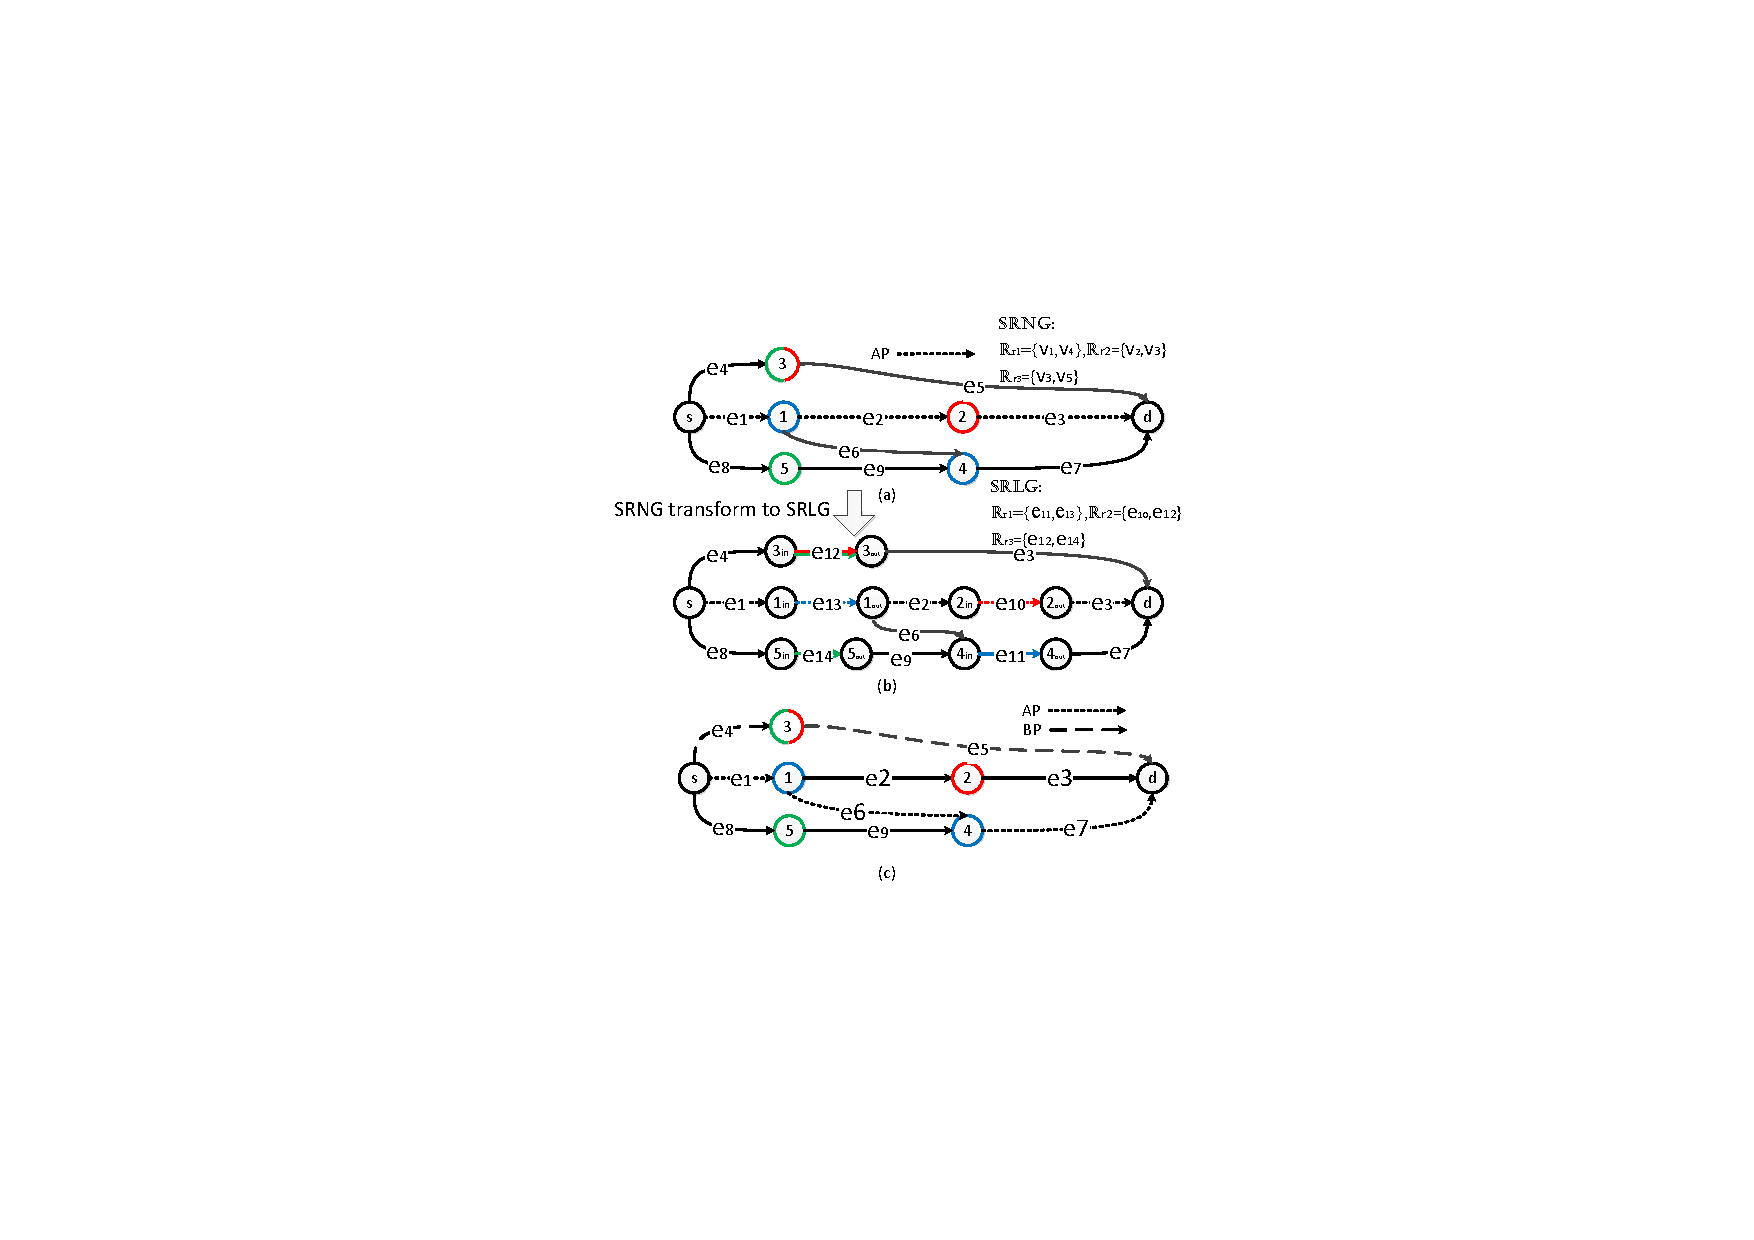
\includegraphics[width=3.0in]{franz/SRNG}
  \caption{(a) A graph with three SRNGs: $\mathbb{R}_{r_1}=\{v_1,v_4\}$,$\mathbb{R}_{r_2}=\{v_2,v_3\}$,$\mathbb{R}_{r_3}=\{v_3,v_5\}$. (b) Transform SRNG to SRLG. $\mathbb{R}_{r_1}=\{v_1,v_4\}\rightarrow \{e_{13},e_{11}\}$,$\mathbb{R}_{r_2}=\{v_2,v_3\}\rightarrow \{e_{10},e_{12}\}$,$\mathbb{R}_{r_3}=\{v_3,v_5\}\rightarrow \{e_{12},e_{14}\}$. (c) AP and BP in the graph.}\label{fig:SRNG}
  \label{fig:SRNG}
\end{figure}
%\begin{figure}[tp]
%  \centering
%  % Requires \usepackage{graphicx}
%  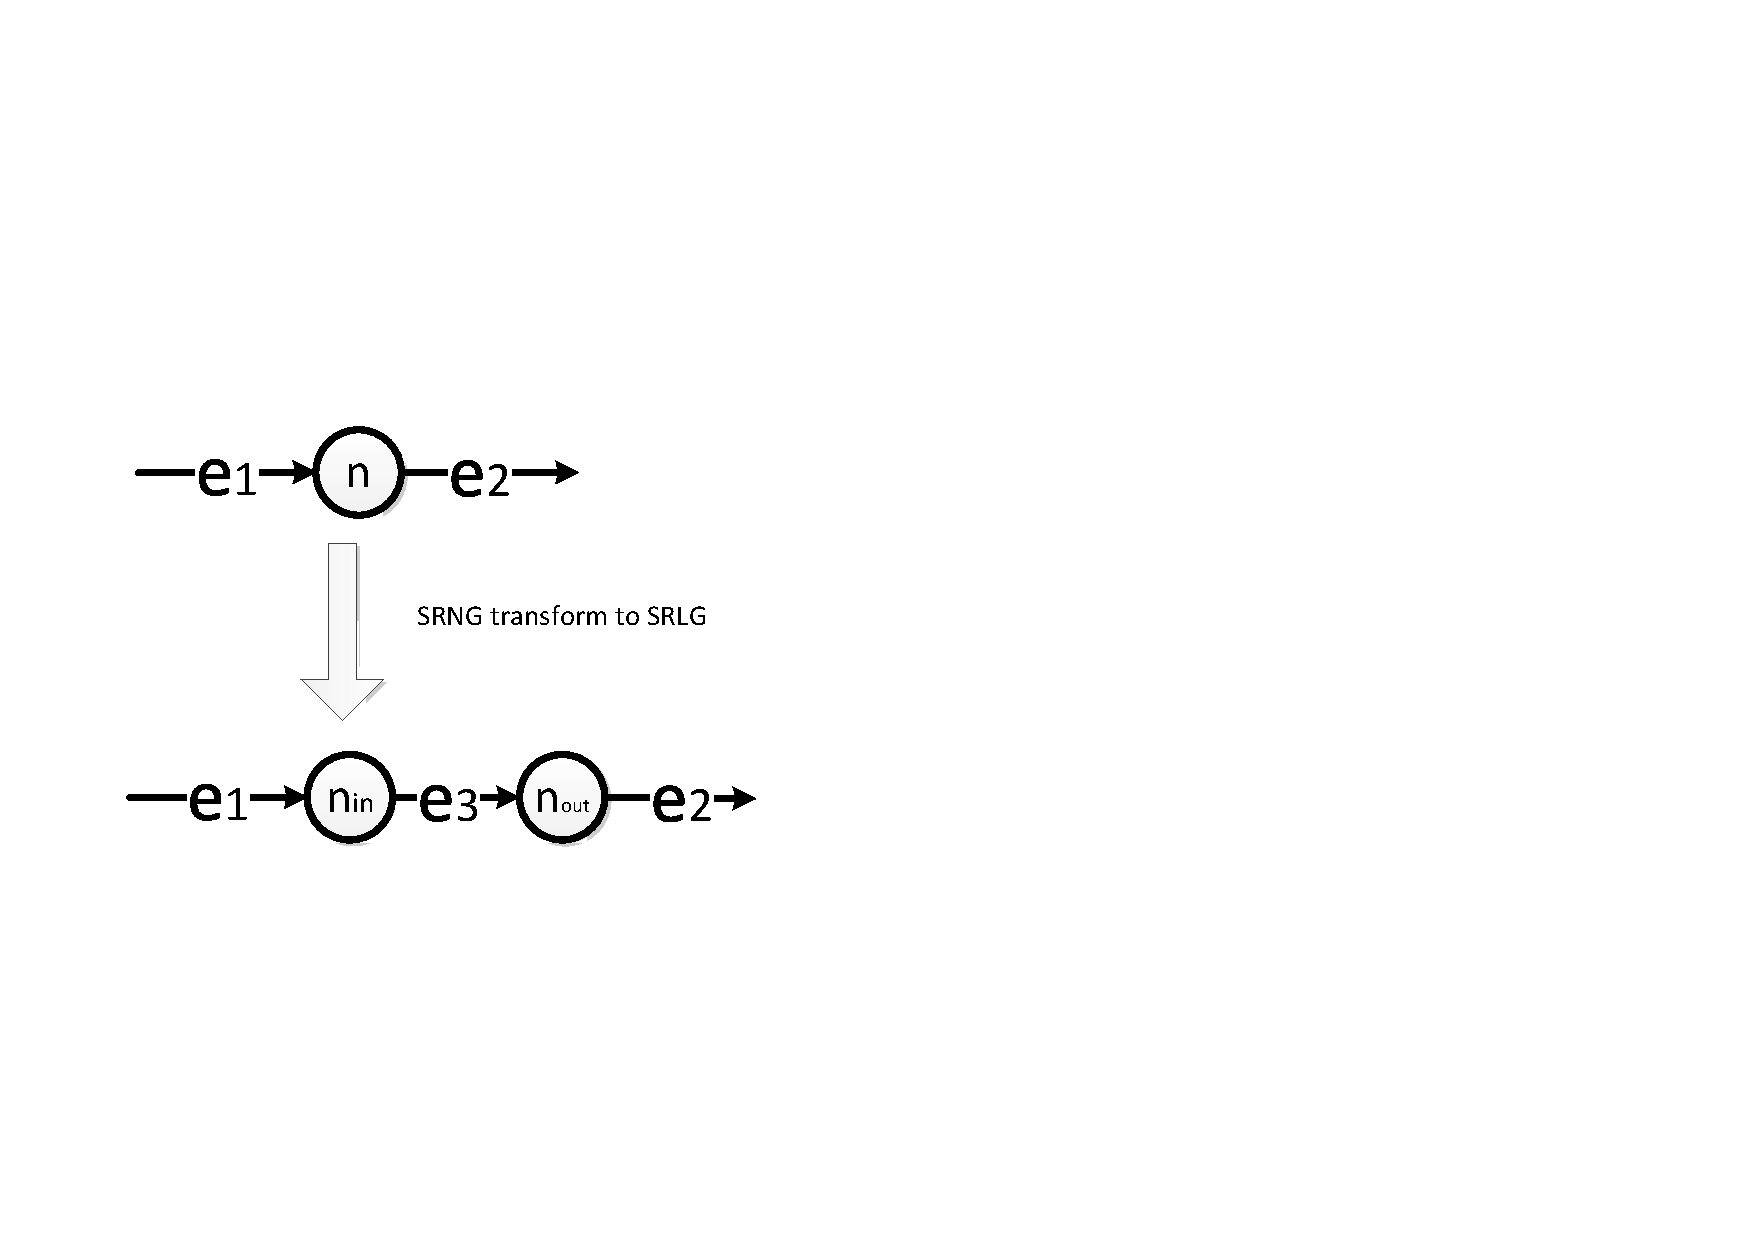
\includegraphics[width=2.0in]{franz/node2edge}
%  \caption{SRNG transform to SRLG. $\mathbb{R}_{r}=\{v_n,\ldots\}\rightarrow \{e_{3},\ldots\}$}\label{fig:node2edge}
%  \label{fig:node2edge}
%\end{figure}


%\subsection{DOMAIN-DISJOINT PATHS}
%\revtao{The domain-disjoint paths problem is formally defined as follows:Given a directed network $G(\mathbb{V},\mathbb{E},\mathbb{D},\mathbb{L})$ of a set $\mathbb{D}$ of $|\mathbb{D}|$ domains, a set $\mathbb{L}$ of $|\mathbb{L}|$ weighted inter-domain links, a set $\mathbb{V}$ of $|\mathbb{V}|$ nodes, a set $\mathbb{E}$ of $|\mathbb{E}|$ weighted links, two special nodes $s,d\in\mathbb{V}$, and an integer $k>0$. Each domain $d\in\mathbb{D}$ consists of a set of nodes $\mathbb{V}_d\subseteq \mathbb{V}$ and a set of links $\mathbb{E}_d\subseteq \mathbb{E}$ that interconnect the nodes in $\mathbb{V}_d$. Find $k$ paths $P_1,P_2,\ldots,P_k$ from $s$ to $d$, such
%that the paths share no common domains.  In multidomain optical networks, domains may be defined
%based on geographic locations of nodes or administrative
%boundaries. If domains are defined based on
%geography, multiple links within the same domain may fail
%simultaneously due to localized failure events\cite{wang2007impairment}, such as power outages or earthquakes. A domain is a set of nodes and links. generally speaking, the domain-disjoint paths problem is combination of the SRNG disjoint and SRLG disjoint problem, therefore our proposed algorithm is extend to the domain-disjoint paths problem.}

